\documentclass[
  11pt,
  letterpaper,
   addpoints,
   answers
  ]{exam}

\usepackage{../exercise-preamble}

\begin{document}

\noindent
\begin{minipage}{0.47\textwidth}

\includegraphics[width=\textwidth]{../fcfm_die}
\end{minipage}
\begin{minipage}{0.53\textwidth}
\begin{center} 
\large\textbf{Fundamentos de control de sistemas} (EL4111-1) \\
\large\textbf{Clase auxiliar 2} \\
\small Prof.~Roberto Cardenas Dobson\\
\small Prof.~Aux.~Osvaldo Jimenez - Erik Sáez\\
\small Ayudantes.~Simon Arenas- Juan Pablo Baez - Francisco Garces - Sofia Ibarra\\
\end{center}
\end{minipage}

\vspace{0.5cm}
\noindent
\vspace{.85cm}

\begin{questions}
    %%%%%%%%%%%%%%%%%%%%%%%%%%%
    \question Considere el siguiente sistema de control visto en Figura 1. Utilizando el método del lugar de la raíz, responda las siguientes preguntas:
    \begin{figure}[h]
        \centering
        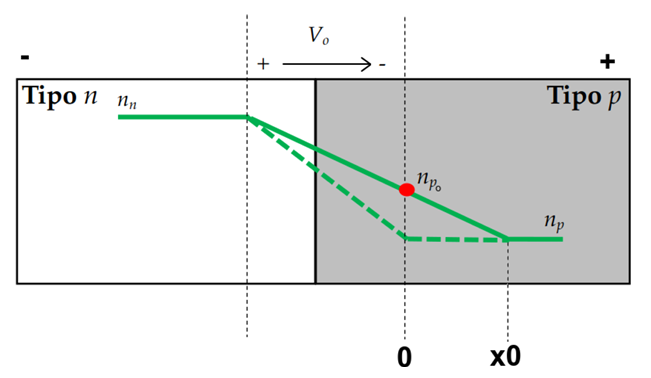
\includegraphics[width=0.7\textwidth]{Auxiliar_2_11}
        \caption{Diagrama de bloques}
    \end{figure}
    \begin{enumerate}
        \item Identifique los puntos en el LGR donde la respuesta del sistema a lazo cerrado no sobrepasará el valor de referencia de entrada con un mínimo tiempo de establecimiento (asuma entrada escalón). Encuentre el valor de \(K_T\) en función de la ganancia \(K_A\) en esos puntos. Además, explique las condiciones de módulo y de ángulo que utiliza durante el desarrollo.
        \item Repita el análisis anterior, pero considerando que la respuesta ahora tiene un \(\xi=0.707\) en la respuesta a lazo cerrado. De manera análoga, explique las condiciones de módulo y de ángulo que utiliza en su desarrollo.
    \end{enumerate}
%%%%%%%%%%%%%%%%%%%%%%%%%%%
\begin{solution}
    \subsection*{Resolución 1.1}
    En primera instancia, debemos encontrar el LGR que representa el diagrama de control. Para ello, debemos analizar la función de transferencia a lazo abierto del sistema, con el fin de encontrar los polos y ceros del mismo. Dado que la forma que tiene el diagrama no es tan intuitiva para resolver, resolvemos el lazo interno para que resulte en una multiplicación de bloques en serie. De esta forma, utilizando la función de transferencia de lazo cerrado:
    \begin{align}
        \frac{G(s)}{1+G(s)H(s)} &= \frac{\frac{1}{s+1}}{1+K_T \cdot \frac{1}{s+1}} \nonumber\\
        &= \frac{\frac{s+1}{s+1}}{s+K_T +1} \nonumber \\
        &= \frac{1}{s+K_T+1} \label{eq1}
    \end{align}
    
    Utilizando lo encontrado en (\ref{eq1}) podemos encontrar la función de transferencia a lazo abierto, multiplicando los bloques del lazo directo:
    \begin{align}
        G(s)H(s) &= \frac{K_A}{s(s+K_T+1)} \label{eq2}
    \end{align}
    
    A partir de (\ref{eq2}), podemos deducir que los polos se encuentran en \( s_1 = 0 \) y \( s_2 = -K_T -1 \). Con lo anterior, procedemos a calcular los componentes del LGR:
    \begin{enumerate}
        \item \textbf{Número de asíntotas: }El número de asíntotas estará dado por la resta entre el número de polos \( N_p \) y el número de ceros \( N_z \). De esta forma, \( N^\circ_A = N_p - N_z = 2 - 0 = 2 \).\\
        \item \textbf{Posición de las asíntotas: } la posición de las asíntotas está dada por la expresión (\ref{eq3}):
        \begin{align}
            \sigma_A &= \frac{\Sigma \sigma_p - \Sigma \sigma_z}{N_p - N_z} \label{eq3}
        \end{align}
        donde \( \sigma_p \) es la posición de los polos y \( \sigma_z \) la posición de los ceros. De esta forma:
        \begin{align}
            \sigma_A &= \frac{0 + (-K_T - 1) - 0}{2 - 0} \nonumber\\
            &= -\frac{(K_T + 1)}{2} \nonumber
        \end{align}
        \item \textbf{Ángulo de las asíntotas: } el ángulo de las asíntotas está dado por la expresión (\ref{eq4}):
        \begin{align}
            \sphericalangle_A &= \frac{(2k+1)}{N_p - N_z}\pi \quad k \in \{0,1,...,N_p - N_z - 1 \} \label{eq4}
        \end{align}
        Considerando que \( N_p - N_z = 2 \), se tendrá que \( k \in \{0,1\} \). Luego, los ángulos de las asíntotas serán \( \sphericalangle_A = \left\{\frac{\pi}{2},\frac{3\pi}{2}\right\} \).
        \item \textbf{Puntos de arranque: }para obtener los puntos de arranque, reescribimos la ganancia del sistema en función de los términos de la ecuación característica. De esta forma:
        \begin{align}
            1 + KG(s)H(s) &= 0 \nonumber\\
            1 + K\frac{K_A}{s(s+K_T+1)} &= 0 \nonumber\\
            s(s+K_T+1) + K(s)K_A &= 0 \implies  \boxed{K(s) = \frac{-s(s+K_T+1)}{K_A}} \label{eq5}
        \end{align}
        Luego, imponiendo \( s = \sigma + j0 \), derivamos la expresión (\ref{eq6}) e igualamos a 0. De esta forma:
        \begin{align}
            \frac{\partial K(\sigma)}{\partial \sigma} &= 0 \nonumber\\
            \frac{\partial}{\partial \sigma}\Big( \frac{-\sigma(\sigma+K_T+1)}{K_A} \Big) &= 0 \nonumber\\
            \frac{(-2\sigma-K_T -1)}{K_A} &= 0 \implies \boxed{\sigma = -\frac{K_T + 1}{2}} \label{eq6}
        \end{align}
        De esta forma, podemos concluir que el LGR del sistema es aquel que se muestra a continuación:
        \begin{center}
            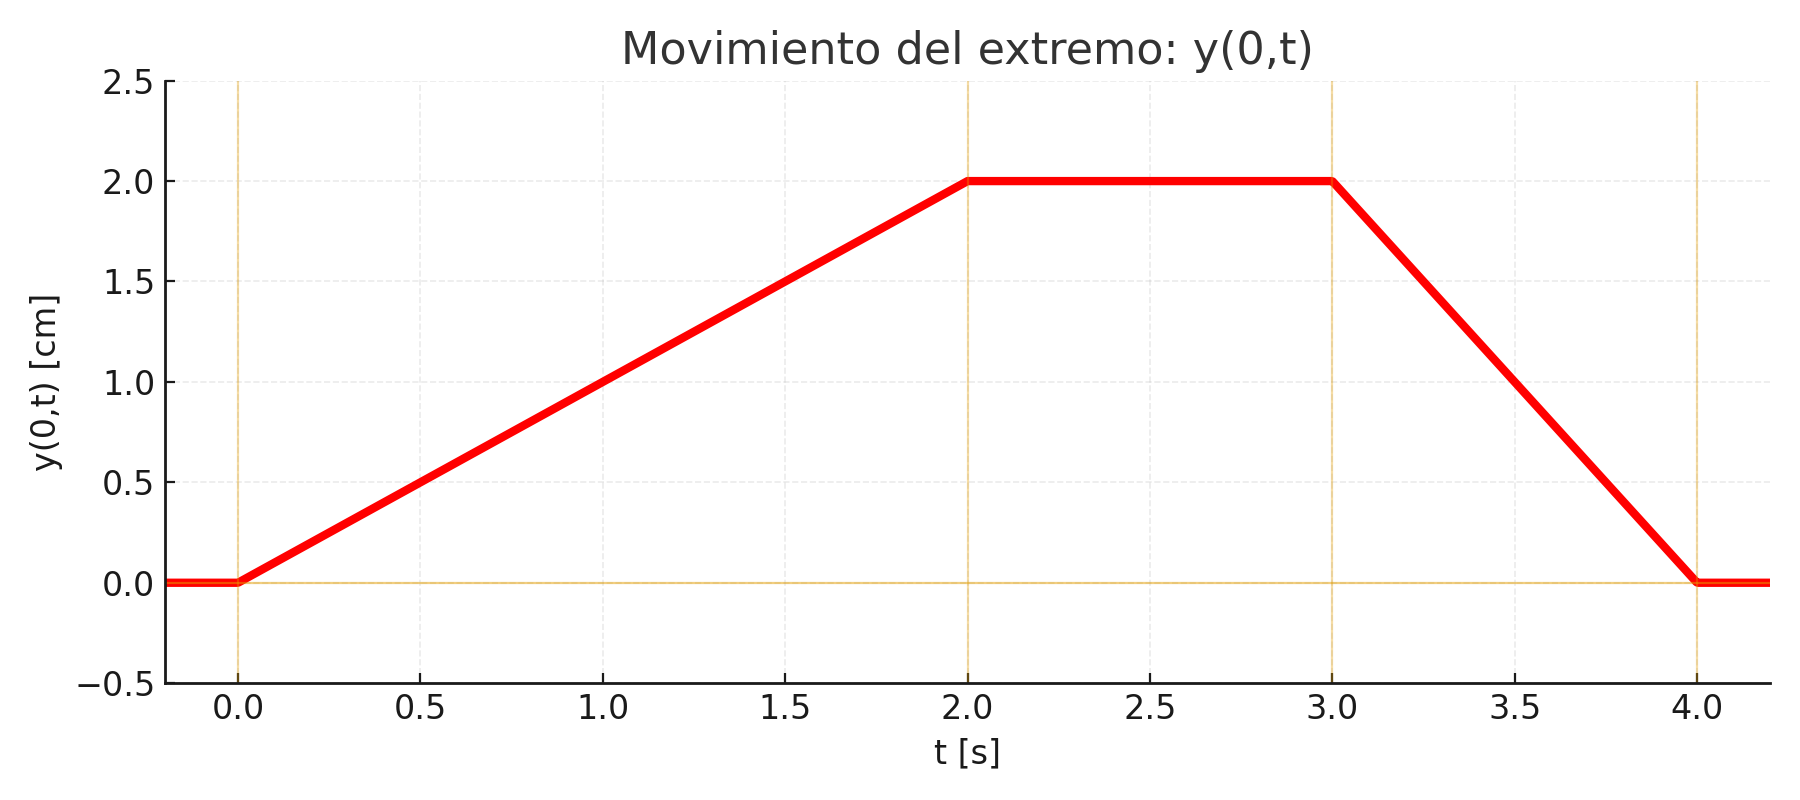
\includegraphics[width=0.5\textwidth]{Auxiliar_2_14}
          \end{center}
    \end{enumerate}
    Notar que los polos de lazo cerrado se podrán mover únicamente por los lugares donde hay LGR, en dirección hacia las asíntotas. Recordar que la cantidad de polos de lazo abierto es la misma que de polos de lazo cerrado. \\

    El enunciado nos pide identificar los puntos del LGR donde la respuesta no sobrepasará el valor de referencia de entrada. En este sentido, lo anterior sugiere que debemos tener un \( \xi \) tal que la respuesta sea lo suficientemente amortiguada como para que la respuesta no sobrepase la referencia. Con esto en mente, se puede concluir que el coeficiente que permite lograr lo anterior es \( \xi = 1 \). Notar que además el enunciado pide lograr el mínimo tiempo de establecimiento (el cual pertenece al tiempo de establecimiento al \( 2\% \)). Dicho tiempo está dado por la expresión:
    \begin{align}
        t_s ^{2\%} &= \frac{4}{\xi \omega_n} \label{eq7}
    \end{align}
    donde \( \xi \) es el coeficiente de amortiguamiento y \( \omega_n \) es la frecuencia natural. Dado que \( \xi = 1 \), \( t_s ^{2\%} = \frac{4}{\omega_n} \). Si revisamos bien el valor del tiempo de establecimiento, podremos notar que este depende únicamente de la frecuencia natural del polo, puesto que el coeficiente de amortiguamiento es unitario. De esta forma, el \( t_s \) será mínimo mientras mayor sea \( \omega_n \). Si recordamos la definición del coeficiente de amortiguamiento, este se puede entender como el coseno del ángulo que describe un polo. Así, si \( \xi = 1 \), entonces \( \cos(\theta) = 1 \), por lo que \( \theta = 0^{\circ} \). Esto quiere decir que el ángulo que describe el polo respecto al eje real es nulo, por lo que la única posibilidad es que el polo de lazo cerrado sea puramente real.
    Por último, recordando que necesitamos maximizar \( \omega_n \) para minimizar \( t_s ^{2\%} \), lo único que nos queda es ver dónde se puede ubicar el polo. Dado que este solo se puede mover por el eje real, el único valor que puede tomar es el que se encuentra en la posición de arranque de las mismas. Esto es puesto que el polo no se puede mover verticalmente por las asíntotas, dado que no puede tener un ángulo distinto de \( 0^{\circ} \) respecto al eje real (es decir, el coeficiente de amortiguamiento unitario limita su movimiento al eje real). Además, el valor de su frecuencia natural es el máximo que se puede encontrar para todas las combinaciones del LGR. Recordar que \( \omega_n \) se define como la distancia del polo al origen).\\

Con el argumento anterior, determinamos que el polo de lazo cerrado (y por ende el punto de diseño) se encuentra en \( s^{*}=-\frac{(K_T+1)}{2} \). De esta forma, utilizando la condición de módulo, tendremos que:

\begin{align}
    K_A &= \left|\frac{1}{\frac{1}{s(s+K_T + 1)}}\right|_{s=s^*} \nonumber \\
    K_A &= \left|s(s+K_T + 1)\right|_{s=s^*} \nonumber\\
    K_A &= \left|-\frac{(K_T+1)}{2}\left(-\frac{(K_T+1)}{2} + K_T + 1 \right)\right| \nonumber\\
    K_A &= \left|-\frac{(K_T+1)}{2} \cdot \frac{(K_T + 1)}{2}\right| \nonumber \\
    K_A &= \frac{(K_T+1)^2}{4} \nonumber \\
    4K_A &= (K_T + 1)^2 \implies \boxed{K_T^2 + 2K_T + 1 - 4K_A = 0}\label{eq8} 
\end{align}
Utilizando la fórmula general para obtener (\ref{eq8}):
\begin{align}
    K_T &= \frac{-2 \pm \sqrt{4-4(1-4K_A)}}{2} \nonumber\\
    K_T &= -1\pm 2\sqrt{K_A} \label{eq9}
\end{align}
Notar que por la condición de módulo, \( K_T > 0 \), por lo que escogemos la solución positiva. Finalmente, llegamos a que \( K_T = -1 + 2\sqrt{K_A} \).
\subsection*{Resolución 1.2}
A diferencia del caso anterior, el coeficiente de amortiguamiento no es unitario, por lo que los polos de lazo cerrado que se desean encontrar poseen un ángulo respecto al eje real distinto de 0. En efecto:
\begin{align}
    \xi &= \cos(\theta) \implies \theta = \arccos(\xi) \implies \theta = \arccos(0.707) \implies \theta = 45^\circ \nonumber
\end{align}
De esta forma, podemos intuir que los polos se ubicarán en la posición descrita por el siguiente LGR:
\begin{center}
    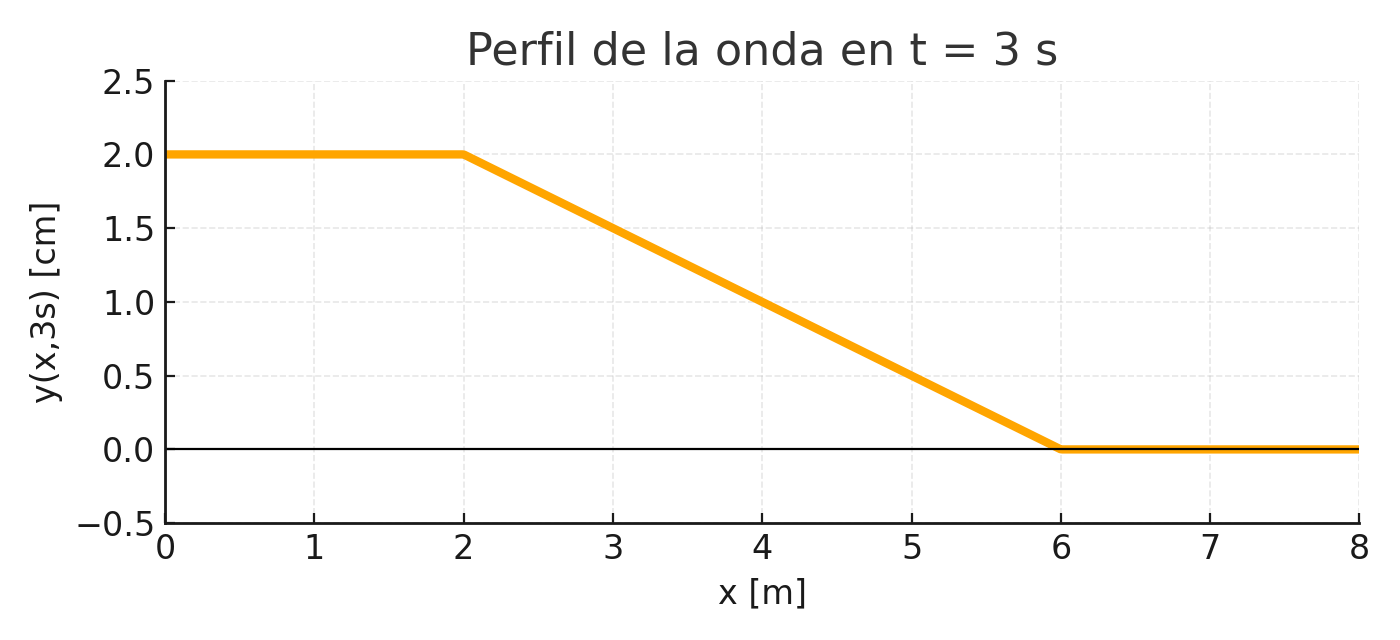
\includegraphics[width=0.5\textwidth]{Auxiliar_2_15}
  \end{center}
Del diagrama se puede deducir que los polos deben encontrarse sobre las asíntotas del LGR. Con un poco de trigonometría se plantea la siguiente relación:
\begin{align}
    \tan(45^\circ) &= \frac{H}{\frac{K_T+1}{2}} \label{eq9}
\end{align}
Dado que \( \tan(45^\circ) = 1 \), se tendrá que \( H = \frac{K_T + 1}{2} \). De esta forma, el punto que cumple con las especificaciones de diseño se encuentra en \( s^* = -\frac{K_T+1}{2} \pm j\frac{K_T + 1}{2} \). Finalmente, evaluamos en la condición de módulo para obtener el valor de \( K_T \):
\begin{align}
    K_A &= \left|\frac{1}{\frac{1}{s(s+K_T + 1)}}\right|_{s=s^*} \nonumber \\
    K_A &= \left|s(s+K_T + 1)\right|_{s=s^*} \nonumber\\
    K_A &= \left|\left( -\frac{(K_T+1)}{2}+j\frac{(K_T+1)}{2}\right) \left(-\frac{(K_T+1)}{2}+j\frac{(K_T+1)}{2} + K_T + 1 \right)\right| \nonumber\\
    K_A &= \left|\left( -\frac{(K_T+1)}{2}+j\frac{(K_T+1)}{2}\right) \left(\frac{(K_T+1)}{2}+j\frac{(K_T+1)}{2}\right)\right| \nonumber \\
    K_A &= \left|-\left(\frac{K_T + 1}{2}\right)^2 - \left(\frac{K_T+1}{2}\right)^2\right| \nonumber \\
    K_A &= 2 \cdot \frac{(K_T + 1)^2}{4} \nonumber \\
    2K_A &= (K_T + 1)^2 \implies \boxed{K_T^2 + 2K_T + 1 - 2K_A = 0} \label{eq10} 
\end{align}
Utilizando la fórmula general, podemos determinar que la ganancia \( K_T \) va a estar dada por:
\begin{align}
    K_T &= \frac{-2\pm \sqrt{4-4(1-2K_A)}}{2} \nonumber\\
    K_T &= -1\pm \sqrt{2K_A} \label{eq11}
\end{align}
De manera análoga al caso anterior, elegimos la solución positiva, puesto que \( K_T > 0 \) por la condición de módulo. Finalmente, \( K_T = 1 + \sqrt{2K_A} \).
\end{solution}
    
    %%%%%%%%%%%%%%%%%%%%%%%%%%%
    %%%%%%%%%%%%%%%%%%%%%%%%%%%
    \question Sea el siguiente diagrama:
    \begin{center}

    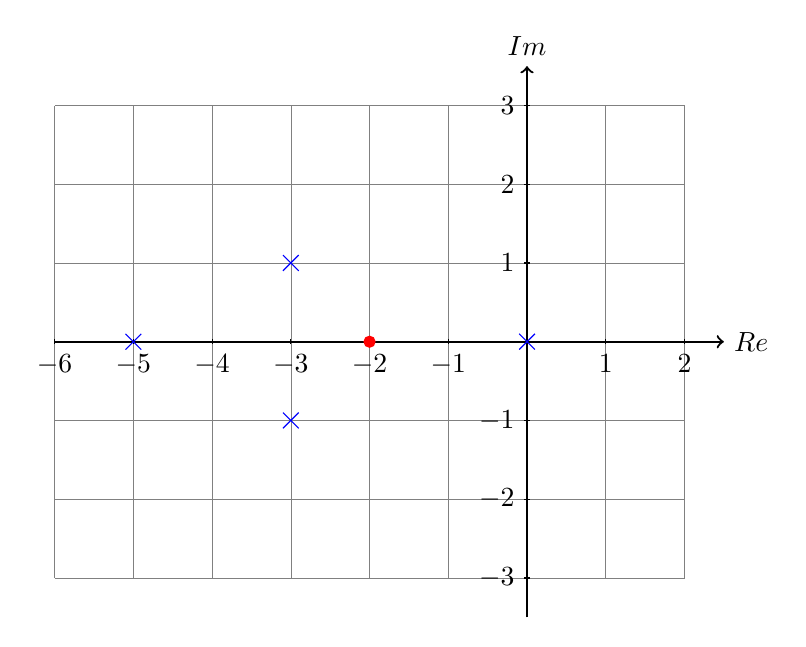
\begin{tikzpicture}
    % Grid setup
    \draw[step=1cm,gray,very thin] (-6,-3) grid (2,3); % Enlarged grid
    
    % Axes
    \draw[thick,->] (-6,0) -- (2.5,0) node[right] {$\text{Re}$}; % Extended x-axis
    \draw[thick,->] (0,-3.5) -- (0,3.5) node[above] {$\text{Im}$}; % Extended y-axis

    % Axis labels
    \foreach \x in {-6,-5,...,2}
      \draw (\x cm,1pt) -- (\x cm,-1pt) node[anchor=north] {\ifnum\x=0 \else $\x$ \fi};
    \foreach \y in {-3,-2,...,3}
      \draw (1pt,\y cm) -- (-1pt,\y cm) node[anchor=east] {\ifnum\y=0 \else $\y$ \fi};

    % Points as blue crosses
    \draw[blue] (0,0) -- ++(-0.1,-0.1) -- ++(0.2,0.2) ++(-0.2,0) -- ++(0.2,-0.2);
    \draw[blue] (-5,0) -- ++(-0.1,-0.1) -- ++(0.2,0.2) ++(-0.2,0) -- ++(0.2,-0.2);
    \draw[blue] (-3,-1) -- ++(-0.1,-0.1) -- ++(0.2,0.2) ++(-0.2,0) -- ++(0.2,-0.2);
    \draw[blue] (-3,1) -- ++(-0.1,-0.1) -- ++(0.2,0.2) ++(-0.2,0) -- ++(0.2,-0.2);

    % Red circle at -2
    \filldraw[red] (-2,0) circle (2pt); % Increased size for visibility
\end{tikzpicture}
\end{center}
    \begin{enumerate}
        \item Encuentre la funcion de transferencia del sistema, con esta informacion , obtenga el lugar de la raiz
        \item ¿Qué ocurre con el lugar de la raíz si el sistema tiene una ganancia negativa? En este caso, encuentre la ganancia crítica para que el sistema se mantenga estable.
    \end{enumerate}
%%%%%%%%%%%%%%%%%%%%%%%%%%%
\begin{solution}
\subsection*{Resolucion 2.1}
Dada la figura de del enunciado , se observa que se tienen 4 polos y un cero, por lo que se tendra:
\begin{itemize}
    \item Polos : $p_1=0$ , $p_2=-3 \pm j$ , $p=-5$.
    \item Cero : $z_1=-2$
\end{itemize}
Con lo que la funcion de transferencia a lazo abierto vendra dada por:
\begin{align}
    H(s)G(s)&=\frac{(s+2)}{s(s+3+j)(s+3-j)(s+5)}\\
     &=\frac{(s+2)}{s(s^2+6s+10)(s+5)}\\
\end{align}
Luego sera de interes encontrar todas las caracteristicas suficientes, tal que nos permitan el obtener el LGR.Comenzamos encontrando los cortes con el eje real , para la cual se utiliza la condicion de angulo en base a la siguiente regla: 
\begin{itemize}
    \item Si la cantidad de polos y ceros es \textbf{PAR}, luego esa zona no pertenecerá al LGR.
    \item Si la cantidad de polos y ceros es \textbf{IMPAR}, luego esa zona pertenecerá al LGR.
\end{itemize}
Se debe tener la precaucion con los polos conjugados,se obtiene por tanto:
\begin{center}
    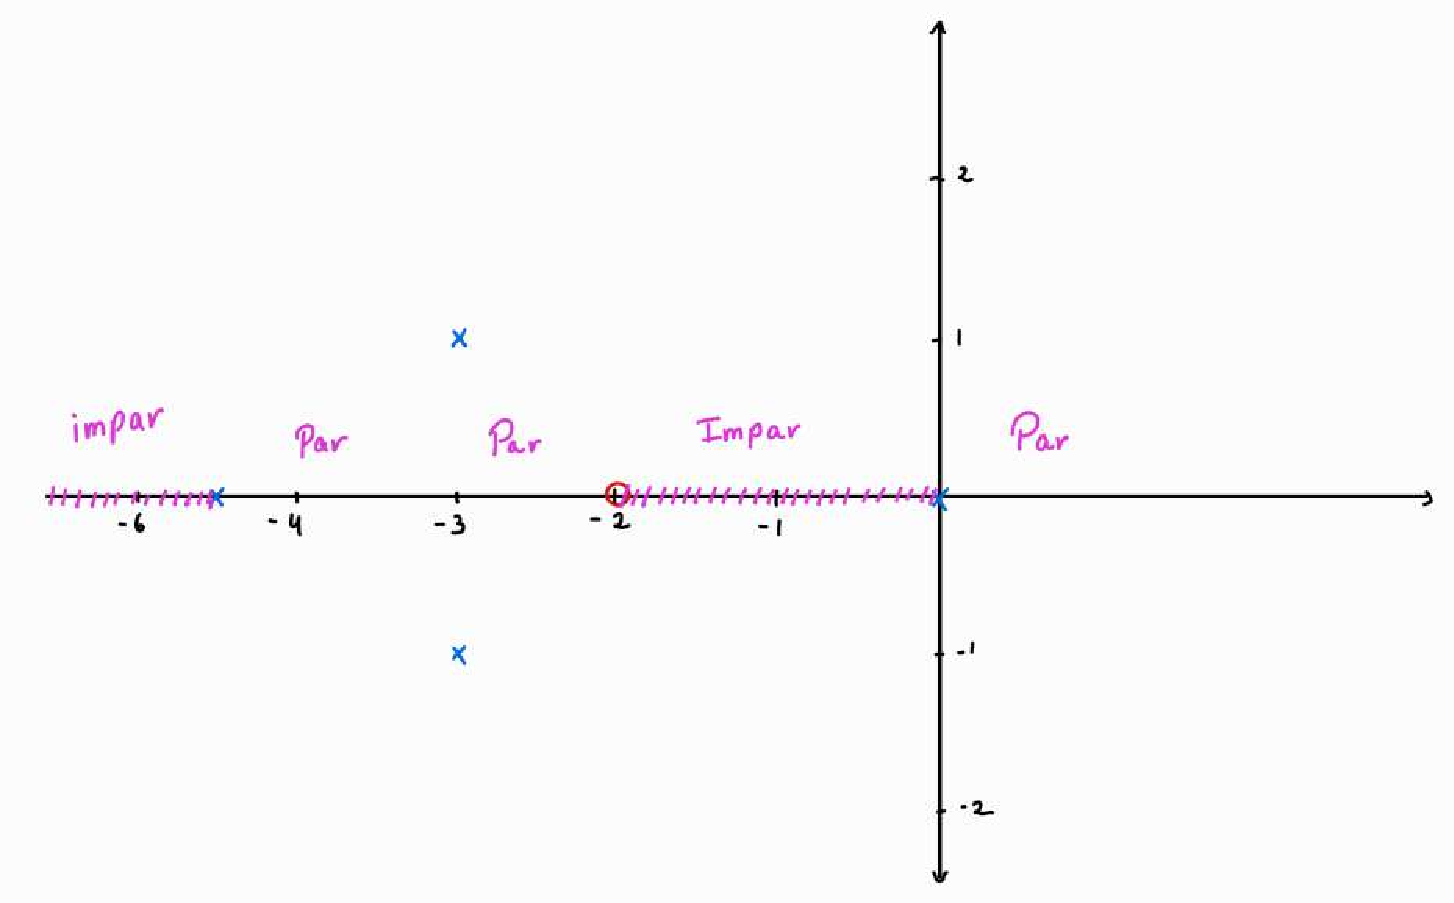
\includegraphics[width=0.5\textwidth]{Auxiliar_2_1}
    \captionof{figure}{Ubicacion de polos de lazo cerrado en zona real}
  \end{center}
Se busca el obtener la ubicacion de las asintotas , para lo cual se utiliza la siguiente formula:
\begin{align}
    \sigma_{a}= \frac{\sum Polos - \sum Ceros}{\# Asintotas} 
\end{align}
Considerando que la asintotas vienen dadas por $\#Asintotas = \#Polos - \#Ceros = 4 - 1 = 3$ se obtiene:
\begin{align}
    \sigma_{a}= \frac{ 0 - 5 -(3 + j) - (3 - j) - (-2)}{3} = -3 
\end{align}
La cual se visualiza en lo siguiente:
\begin{center}
    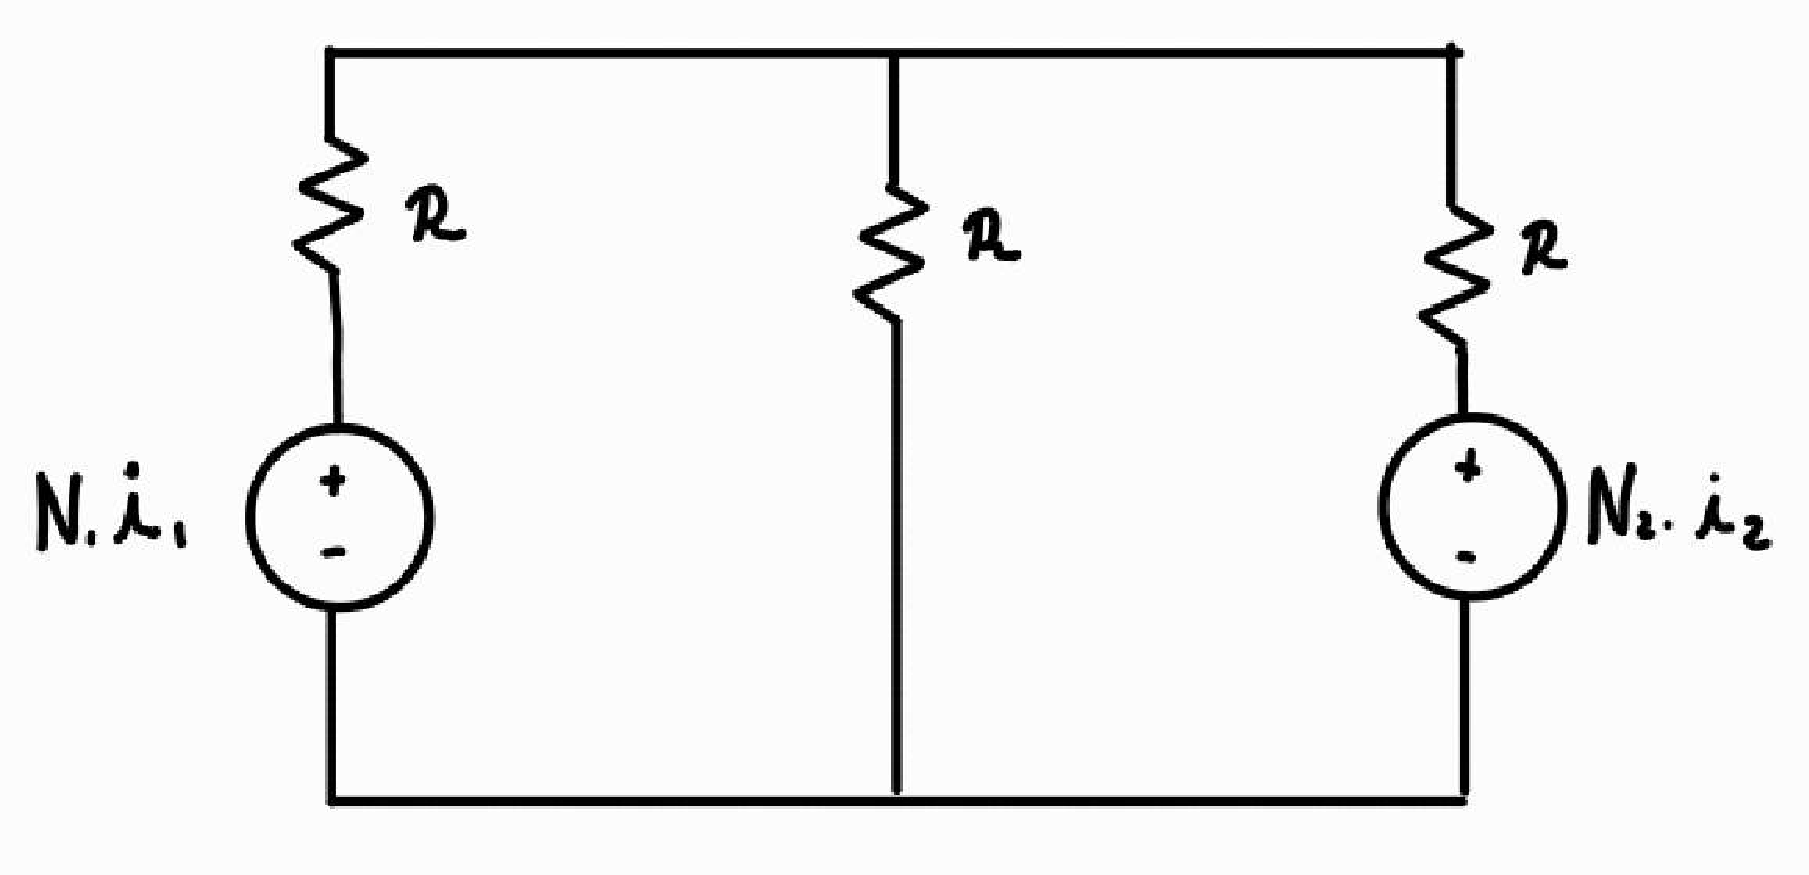
\includegraphics[width=0.5\textwidth]{Auxiliar_2_2}
    \captionof{figure}{Ubicacion de lugar de la asintota}
  \end{center}
Para los angulos asociados a las asintotas tenemos que $k \in \{0,\dots, \#Asintotas -1\}$ con lo que (Para $k>0$):
\begin{align}
    \theta_{k} = \frac{(2k+1)180}{\#Asintotas}
\end{align}
Con lo que se obtiene:
\begin{align}
    \theta_{0} &=  \frac{\pi}{3} \Leftrightarrow 60^{\circ} \\
    \theta_{1} &=  \pi \Leftrightarrow 180^{\circ} \\
    \theta_{2} &=  \frac{5\pi}{3} \Leftrightarrow 300^{\circ} 
\end{align}
Con lo cual:
\begin{center}
    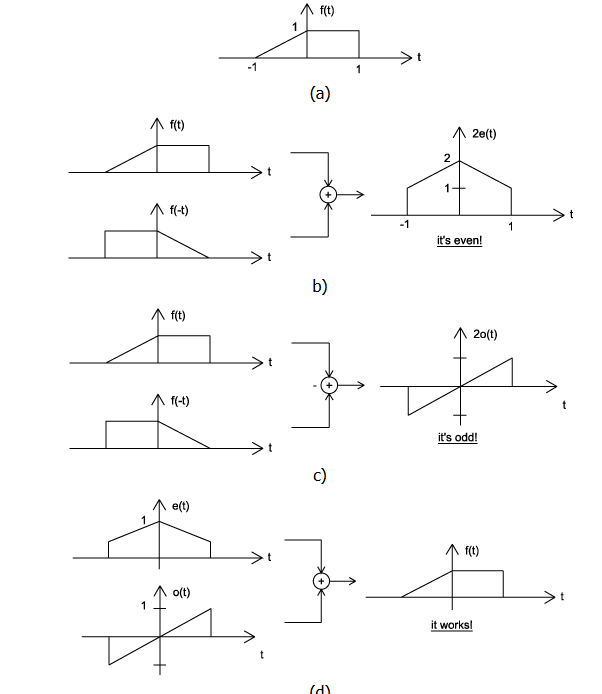
\includegraphics[width=0.5\textwidth]{Auxiliar_2_3}
    \captionof{figure}{Angulos asociados a las asintotas}
  \end{center}
Se debe obtener los valores de llegada o salida, para lo cual se utiliza la expresion de lazo cerrado dada por:
\begin{align}
    1+kG(s)H(s) &= 0\\
    1+ k\frac{(s+2)}{s(s^{2}+6s+10)(s+5)} &= 0\\
    k = \frac{-s(s^{2}+6s+10)(s+5)}{(s+2)}\\
\end{align}
Luego derivamos e igualamos a 0 , con lo que se obtiene que 
\begin{align}
    \frac{dK}{ds} &= \frac{d}{ds} \left( \frac{-s(s^{2}+6s+10)(s+5)}{(s+2)} \right) = 0
\end{align}
Se tiene que $s_{1,2}= -3.7293 \pm 0.29837j$ y $s_{3,4}=-1.2707 \pm 0.8757j$ se observa que ambos son complejos por lo que \textbf{no existe corte con el eje real}.Se debe analizar si esque existe corte con el eje imaginario, por lo tanto:
\begin{align}
    1+kG(s)H(s) &= 0\\
    1+k\frac{(s+2)}{s(s^{2}+6s+10)(s+5)} &= 0\\
    s(s^{2}+6s+10)(s+5)+k(s+2)=0
\end{align}
Dado que nos interesa analizar el corte con el eje real, se impone que $s=j\omega$ con lo que se obtiene:
\begin{align}
    j\omega((j\omega)^{2}+6(j\omega)+10)(j\omega+5)+k(j\omega+2)=0\\
    j\omega( -\omega^{2}+6j\omega+10)(j\omega+5)+k(j\omega+2)=0\\
    \omega^{4}-40\omega^{2}+2k + j(50\omega +k\omega-11\omega^{3})=0
\end{align}
Lo anterior sera valido cuando tanto parte real e imaginaria sean nulas, por lo que igualando se obtiene:
\begin{align}
    \omega^{4}-40\omega^{2}+2k &= 0\\
    50\omega +k\omega-11\omega^{3} &= 0
\end{align}
Luego:
\begin{align}
    \omega_{1,2} &= \pm 4.7385 & k_{1,2}&= 196.99\\
    \omega_{3} &= 0 & k_{3}&= 0
\end{align}
Con lo que la solucion factible corresponde a $\omega_{1,2} = \pm 4.7385$ y $k_{1,2}= 196.99$, dado que $w_{3}$ es infactible dado que es un valor nulo o trivial (Es super importante destacar que la solucion se obtiene considerando $K>0$ , dado que si no se limita esta cantidad, entregara todo el conjunto de soluciones).Finalmente es posible el graficar el lugar geometrico de la raiz el cual vendra dado por lo siguiente:
\begin{center}
    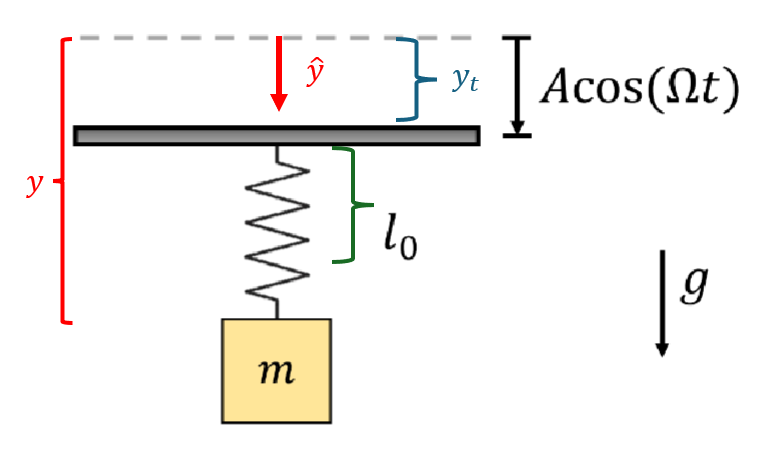
\includegraphics[width=0.5\textwidth]{Auxiliar_2_4}
    \captionof{figure}{Lugar Geometrico de la Raiz}
  \end{center}
\subsection*{Resolucion 2.2}
Dado que se tiene un sistema con ganancia negativa, se tiene que la funcion de transferencia vendra dada por (Considerando que $k>0$):
\begin{align}
    1-kG(s)H(s) &= 0
\end{align}
Con lo que la condicion sera:
\begin{align}
    \angle G(s)H(s) &= 0 \pm 360^{\circ} 
\end{align}
Por lo que notamos que al analizar el corte con el eje real, la condicion que se obtenia antes se invierte, es decir:
\begin{itemize}
    \item Si la cantidad de polos y ceros es \textbf{Impar}, luego esa zona no pertenecerá al LGR.
    \item Si la cantidad de polos y ceros es \textbf{PAR}, luego esa zona pertenecerá al LGR.
\end{itemize}
Por lo que se obtiene lo opuesto a lo ya visto con anterioridad, es decir:
\begin{center}
    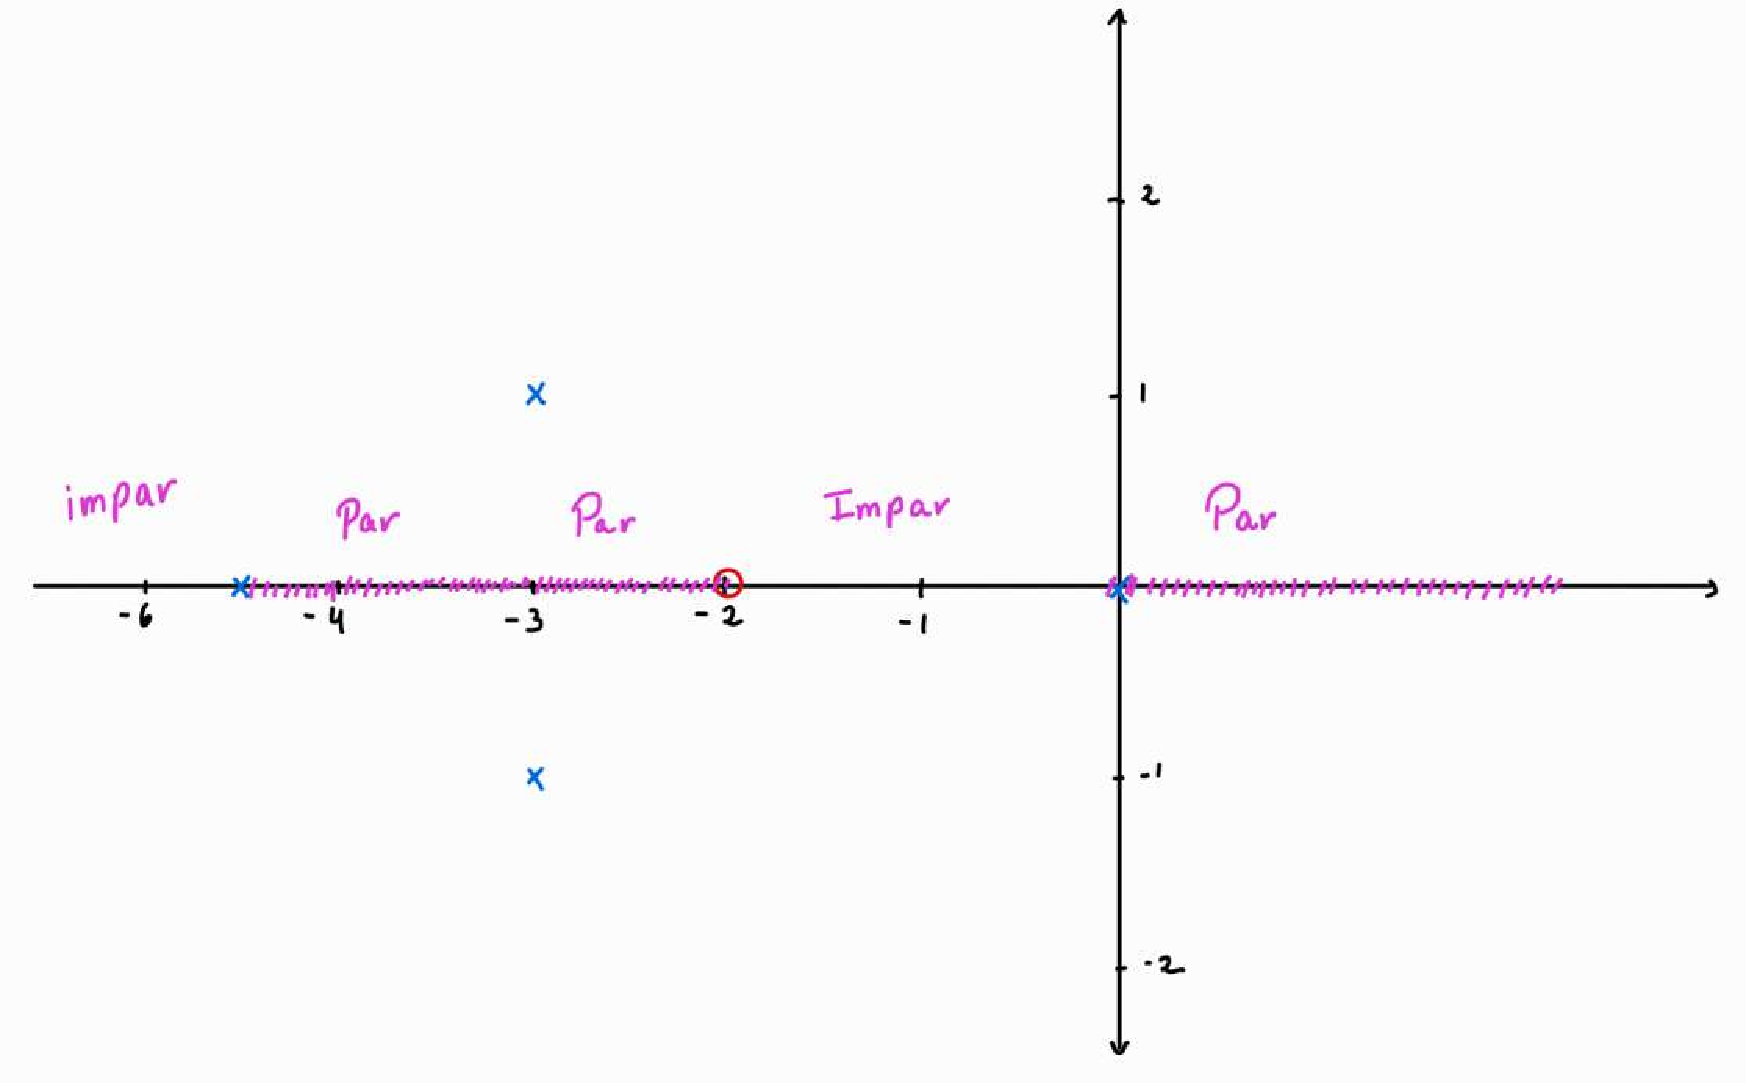
\includegraphics[width=0.5\textwidth]{Auxiliar_2_5}
    \captionof{figure}{Lugar Geometrico de la Raiz}
  \end{center}
Luego la posicion de las asintotas no cambiara, pero si los angulos, estos vendran asociados a los numeros pares, es decir:
\begin{align}
    \theta_{k} = \frac{2k \pi}{\#Asintotas}
\end{align}
Con lo que se obtiene que:
\begin{align}
    \theta_{0} &=   \Leftrightarrow 0^{\circ} \\
    \theta_{1} &=   \frac{2\pi}{3} \Leftrightarrow 120^{\circ} \\
    \theta_{2} &=  \frac{4\pi}{3} \Leftrightarrow 240^{\circ} 
\end{align}
De esta manera al ubicarlos:
\begin{center}
    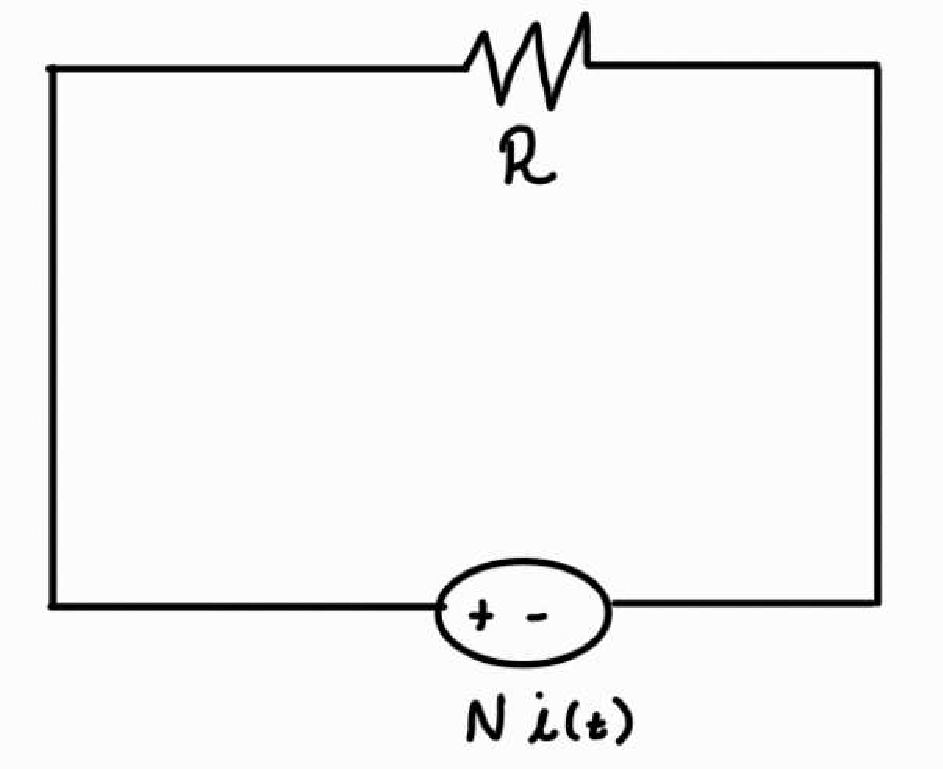
\includegraphics[width=0.5\textwidth]{Auxiliar_2_6}
    \captionof{figure}{Lugar Geometrico de la Raiz}
  \end{center}
Notamos que los valores de llegada o salida \textbf{no se ven afectados por el signo de la ganancia}, por lo que se concluye de manera directa que nuevamente no habra corte en el eje real. Finalmente queda analizar el corte con el eje imaginario , el cual vendra dado por:
\begin{align}
    1-kG(s)H(s) &= 0\\
    1-k\frac{(s+2)}{s(s^{2}+6s+10)(s+5)} &= 0\\
    s(s^{2}+6s+10)(s+5)-k(s+2)=0
\end{align}
Reemplazando por $s=j\omega$ se obtiene:
\begin{align}
    \omega^{4}-40\omega^{2}-2k + j(50\omega -k\omega-11\omega^{3})=0
\end{align}
Que separando parte rteal e imaginaria se obtiene:
\begin{align}
    \omega^{4}-40\omega^{2}-2k &= 0\\
    50\omega -k\omega-11\omega^{3} &= 0
\end{align}
Finalmente se obtienen los valores de $\omega$ y $k$ que son:
\begin{align}
    \omega_{1,2} &= \pm 2.110j & k_{1}&= -98.990
\end{align}
Se observa que son infactibles debido a que $w_{1,2}$ es un valor complejo , por lo que no cortara al eje imaginario, de esta manera podemos graficar el LGR el cual vendra dado por lo siguiente:
\begin{center}
    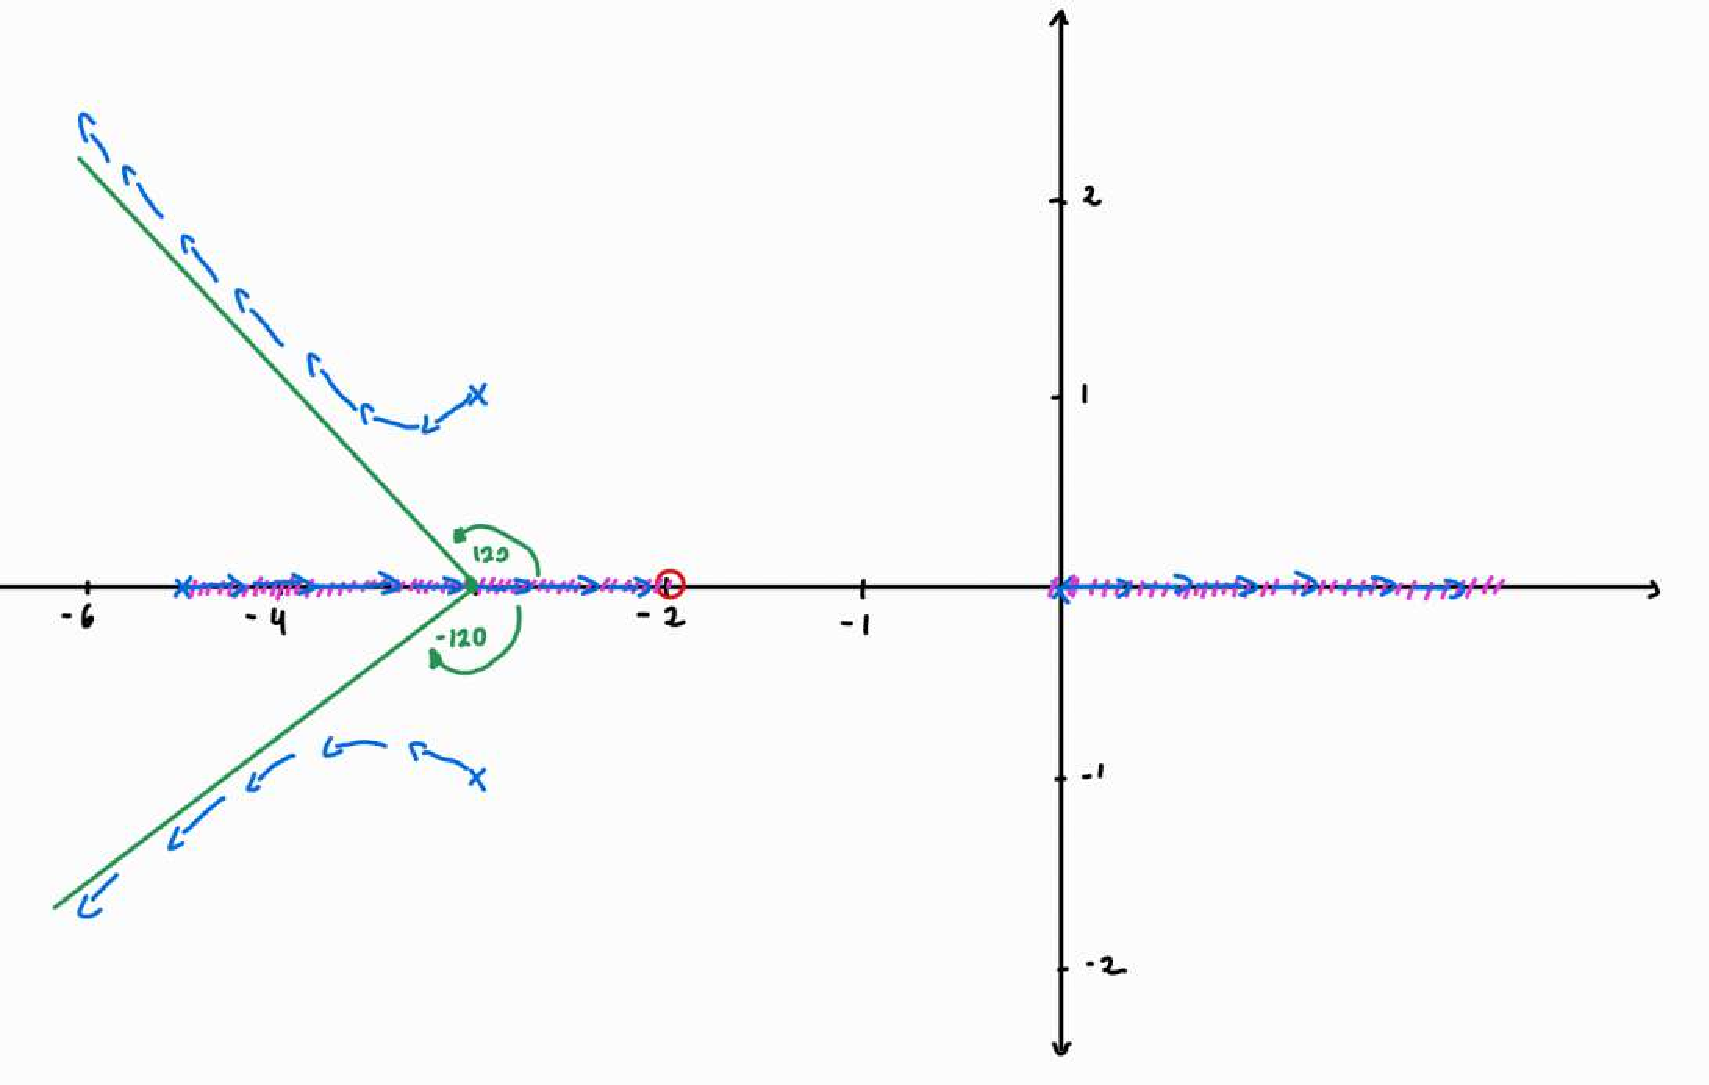
\includegraphics[width=0.5\textwidth]{Auxiliar_2_7}
    \captionof{figure}{Lugar Geometrico de la Raiz}
  \end{center}
\end{solution}
%%%%%%%%%%%%%%%%%%%%%%%%%%%
\question Encuentre los cortes al eje imaginario de la planta:
\begin{align}
    H(s)G(s) = \frac{(s+3)}{s^{2}-s-2}
\end{align}
%%%%%%%%%%%%%%%%%%%%%%%%%%%
\begin{solution}
\subsection*{Resolucion 3.1 (Forma 1)}
Dada la funcion de transferencia de la planta,
\begin{align}
    H(s)G(s) &= \frac{(s+3)}{s^{2}-s-2}\\
             &= \frac{(s+3)}{(s-2)(s+1)}
\end{align}
Con lo que tenemos que los polos de la planta vendran dados por $p_{1} = 2$ y $p_{2} = -1$ y el cero $z_{1} = -3$. Se debe analizar el corte con el eje imaginario, para lo cual se considera el criterio de Routh-Hurwitz,el cual nos permite analizar los rangos de ganancia que permiten la estabilidad del sistema en base a una tabla y los cambios de signos de la misma.Para esto se debe expresar la funcion de transferencia de lazo cerrado en forma polinomica, con lo que se obtiene:
\begin{align}
    1+kG(s)H(s) &= 0\\
    1+k\frac{(s+3)}{(s-2)(s+1)} &= 0\\
    (s-2)(s+1)+k(s+3) &= 0\\
    s^{2}-s-2+ks+3k &= 0\\
    s^{2}+(k-1)s-2+3k &= 0
\end{align}
Luego utilizamos la tabla tal que:
\begin{center}
    \begin{tabular}{|c|cc|}
        \hline
        $s^{2}$ & 1 & -2+3k\\
        $s^{1}$ & k-1 & 0\\
        $s^{0}$ & $\alpha_{1}$ & $\alpha_{2}$\\
        \hline
    \end{tabular}
\end{center}
Donde para obtener los valores de $\alpha_{1}$ y $\alpha_{2}$ se utilizan las formulas asociadas:
\begin{align}
    \alpha_{1} &= \frac{(3k-2)(k-1)-0}{k-1} = (3k-2)\\
    \alpha_{2} &= 0
\end{align}
(Yo suelo utilizar este ayuda memoria para no olvidarme)
\begin{center}
    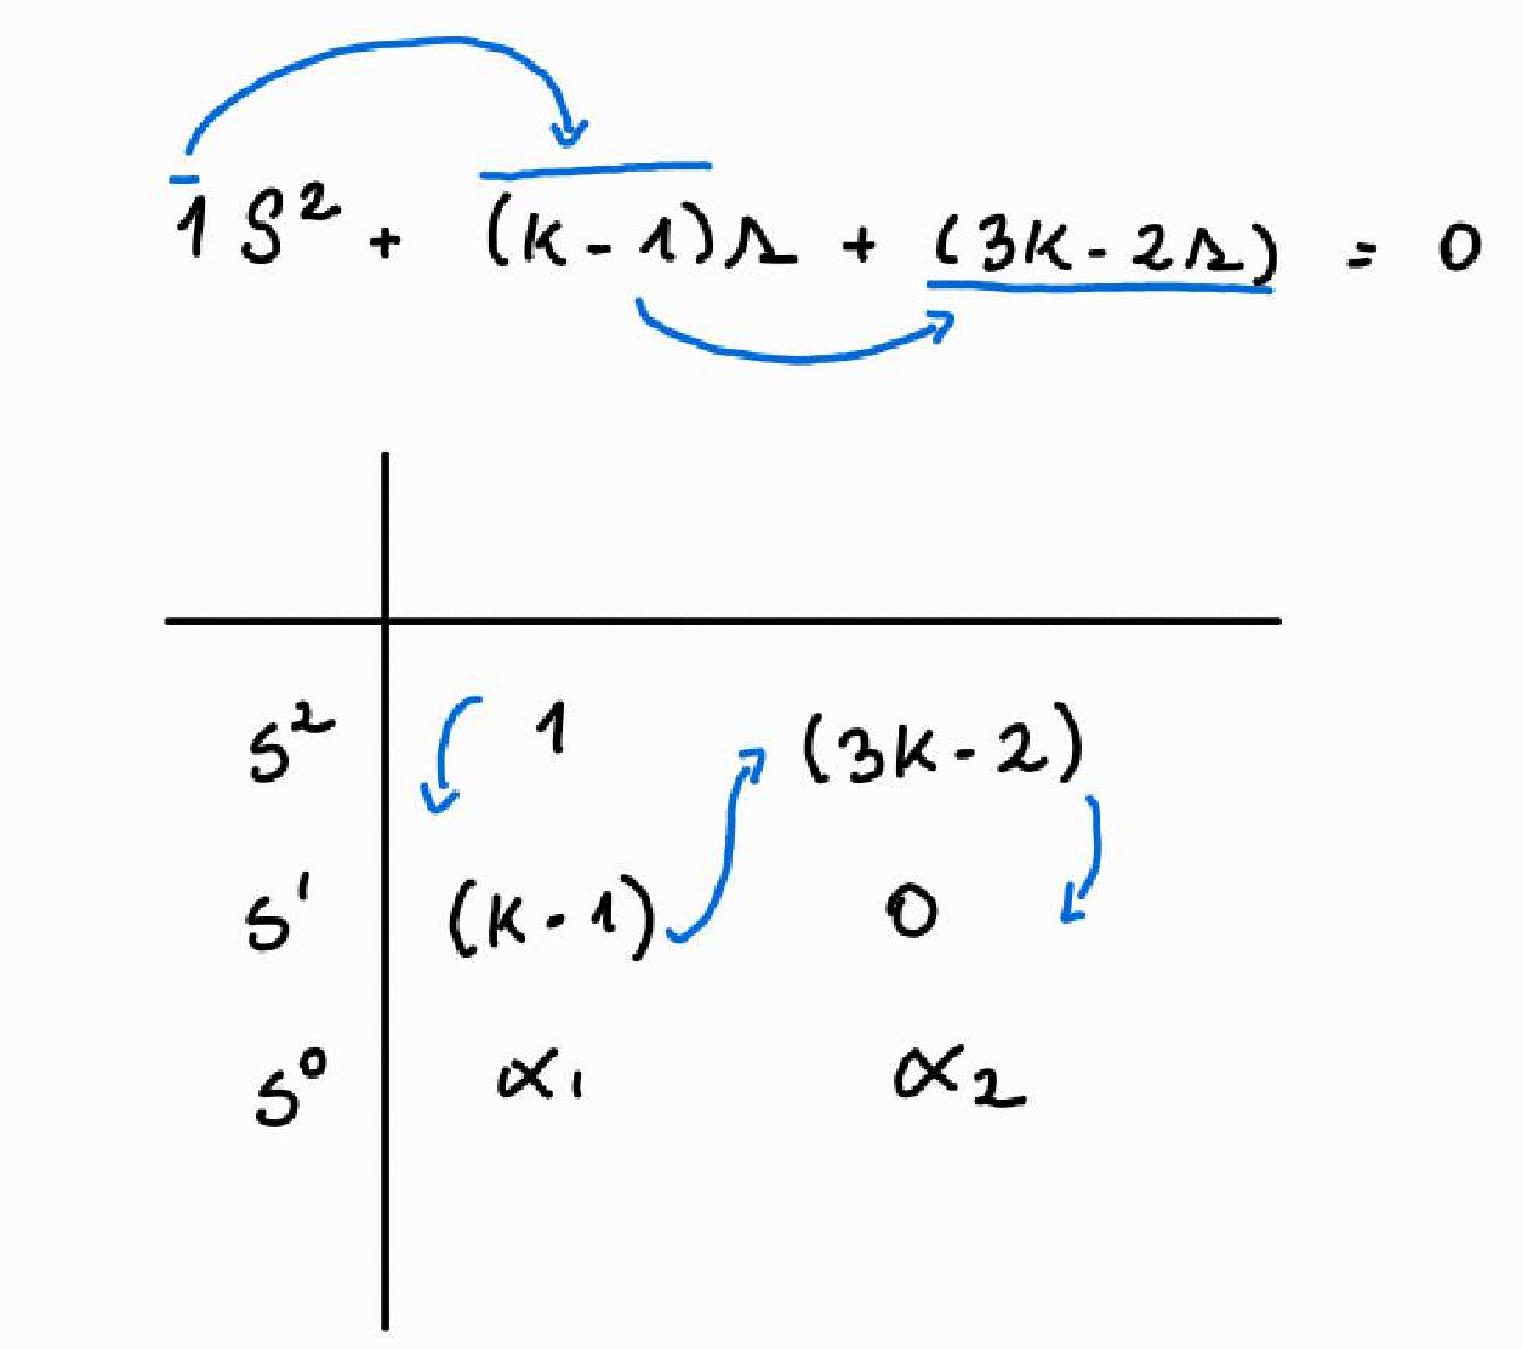
\includegraphics[width=0.3\textwidth]{Auxiliar_2_8}
    \captionof{figure}{La idea es situar en la columna de la izquierda el mayor de grado hasta el menor grado, posteriormente reconocemos los coeficientes del polinomio y trazamos las flechas azules, desde la esquina superior izquierda bajando y luego subiendo hasta completar todo los coeficientes del polinomio (En caso de no haber se rellena con 0).}
  \end{center}
  \begin{center}
    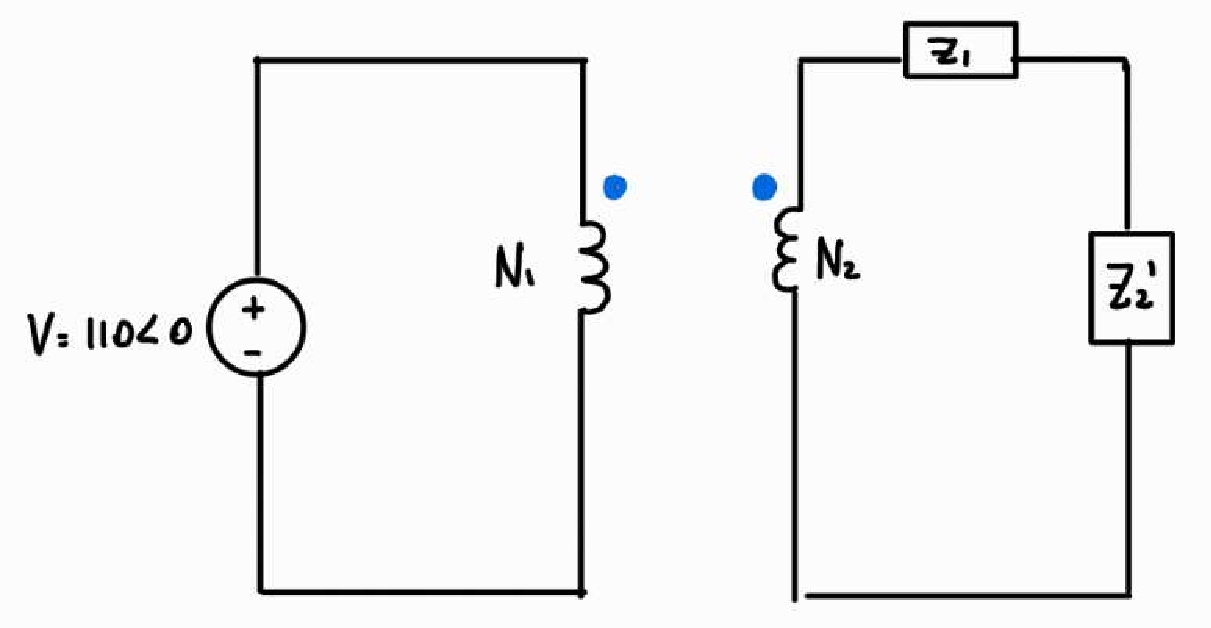
\includegraphics[width=0.55\textwidth]{Auxiliar_2_9}
    \captionof{figure}{Una vez ubicados los coeficientes se deben calcular los coeficientes, por lo que por ejemplo para calcular $\alpha_{1}$ se utiliza el termino superior y se realiza un \textit{Pivote} y luego se realizan las multiplicaciones diagonales y se restan y se dividen por el \textit{Pivote}.}
  \end{center}
  \begin{center}
    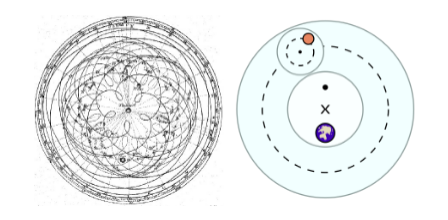
\includegraphics[width=0.55\textwidth]{Auxiliar_2_10}
    \captionof{figure}{Para $\alpha_{2}$ se utiliza el mismo procedimiento}
  \end{center}
Esta metodologia utilizaba para no olvidarme, pero siempre es a criterio personal.Luego tenemos que la matriz vendra dada por:
\begin{center}
    \begin{tabular}{|c|cc|}
        \hline
        $s^{2}$ & 1 & 3k-2\\
        $s^{1}$ & k-1 & 0\\
        $s^{0}$ & $3k-2$ & 0\\
        \hline
    \end{tabular}
\end{center}
El criterio de Routh-width se basa en analizar la segunda columna, para la cual el cambio de signo es equivalente a entrar a zona donde este sea inestable, o equivalentemente cruze el semiplano derecho, por lo que se debera cumplir que en todo momento la primera columna sea positiva, por lo que se obtiene un intervalo vendra dado por (Es importante destacar que este analisis se realiza considerando que $k>0$):
\begin{align}
    k-1 &> 0\\
    3k-2 &> 0
\end{align}
Con lo que se debe cumplir en simultaneo que $k>1$ y $k>\frac{2}{3}$, por lo que se obtiene que $k>1$ cumplira ambas condiciones que permitira la estabilidad .Finalmente se obtiene que el corte con el eje imaginario vendra dado por los momentos en que existe cambio de signo, por lo que estos correpsonden a $k_{1} = \frac{2}{3}$ y $k_{2}=1$, con lo que reemplazando sobre la funcion de transferencia de los polos de lazo cerrado se obtiene que:
\subsubsection*{Caso 1: $K=\frac{2}{3}$}
\begin{align}
    s^{2}+(k-1)s-2+3k &= 0\\
    (jw)^{2}+(k-1)jw-2+3\cdot \left|\frac{2}{3}\right| &= 0\\
    -w^{2}+jw\frac{-1}{3} +0 &= 0\\
\end{align}
Luego igualamos separamos parte real e imaginaria y obtenemos que:
\begin{align}
    -w^{2} &= 0\\
    -\frac{1}{3}w &= 0
\end{align}
Con lo que se obtiene que $s=0$, por lo que el corte se obtiene en el origen.
\subsubsection*{Caso 2: K=1}
Analogamente tenemos que:
\begin{align}
    s^{2}+(k-1)s-2+3k &= 0\\
    (jw)^{2}+(k-1)jw-2+3\cdot 1 &= 0\\
    -w^{2}+jw(1-1) -2+3 &= 0\\
\end{align}
Luego tenemos solo parte real,:
\begin{align}
    w^{2} &= \pm 1
\end{align}
De esta manera tenemos que los cortes se cumplen para $s= \pm j$.
\subsection*{Resolucion 3.2 (Forma 2)} 
Otra condicion que se utilizara con mucha mas frecuencia es a la condicion de angulo , la cual vendra dada por:
\begin{align}
    \angle \sum \Theta_{polos} - \sum \Theta_{ceros} = \pm 180^{\circ} + n360^{\circ} 
\end{align}
De esta manera tenemos que encontrar los angulos asociados a los polos y ceros deberan cumplir tal condicion, pero ademas deberemos considerar que s=jw , dado nos interesa el corte en el eje real que cumpla dicha condicion de angulo.Retomando la funcion de transferencia:
\begin{align}
    H(s)G(s) &= \frac{(s+3)}{s^{2}-s-2}\\
             &= \frac{(s+3)}{(s-2)(s+1)}
\end{align}
Tenemos luego que existe $p_{1}=-1$,$p_{2}=2$ y $z_{1}=-3$ , con lo que luego tenemos que se debe cumplir que:
\begin{align}
    \theta_{z_{1}} - (\theta_{p_{1}} + \theta_{p_{2}}) &= 180
\end{align}
Que graficamente correspondera a lo siguiente (Debemos recordar siempre como es la apertura de los angulos):
\begin{center}
    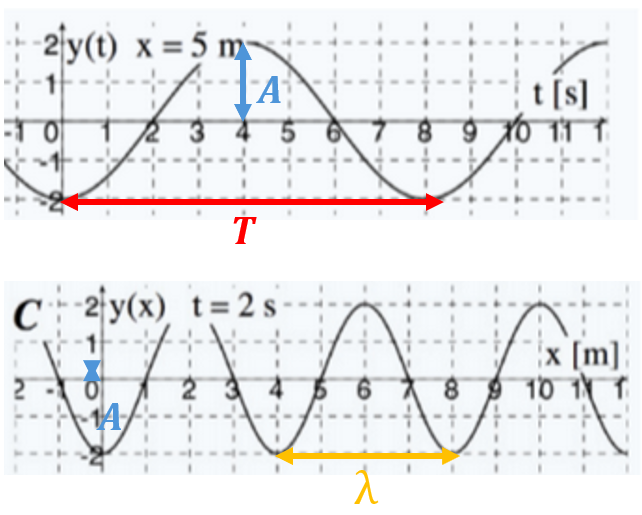
\includegraphics[width=0.55\textwidth]{Auxiliar_2_13}
    \captionof{figure}{Recordatorio de como se miden los angulos para algun punto que pertenece al LGR}
  \end{center}
  \begin{center}
    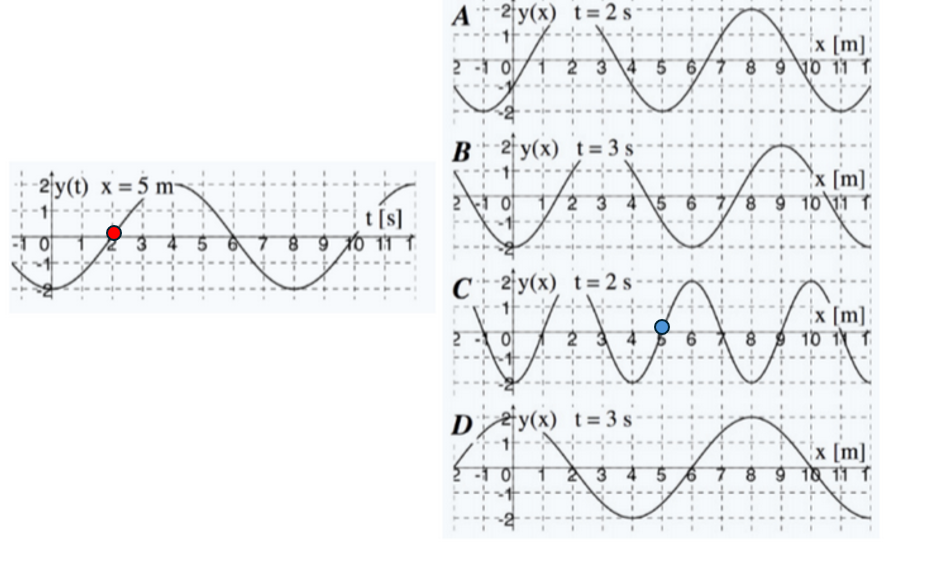
\includegraphics[width=0.55\textwidth]{Auxiliar_2_12}
    \captionof{figure}{Angulos para la funcion de transferencia vista con anterioridad} 
  \end{center}
\begin{align}
    tan(\theta_{p_{1}})&= \frac{w}{1}\\
    tan(\theta_{p_{2}})&= \frac{w}{2}\\
    tan(\theta_{z_{1}})&= \frac{w}{3}
\end{align}
Con lo que sus respectivos angulos corresponderan a:
\begin{align}
    \theta_{p_{1}} &= atan(\frac{w}{1})\\
    \theta_{p_{2}} &= 180 - atan(\frac{w}{2})\\
    \theta_{z_{1}} &= atan(\frac{w}{1})
\end{align}
Con lo que reemplazando en la condicion de angulo se obtiene que:
\begin{align}
    atan(\frac{w}{3}) - (atan(\frac{w}{1}) + 180 - atan(\frac{w}{2})) &= 180\\
    atan(\frac{w}{3}) - atan(\frac{w}{1}) - 180 + atan(\frac{w}{2}) &= 180\\
    atan(\frac{w}{3}) - atan(\frac{w}{1}) + atan(\frac{w}{2}) &= 360
\end{align}
Donde ademas sabemos que 360 es equivalente a 0, por lo que se obtiene que:
\begin{align}
    atan(\frac{w}{3}) - atan(\frac{w}{1}) + atan(\frac{w}{2}) &= 0
\end{align}
Luego queda por resolver la ecuacion , la cual entrega tres soluciones:
\begin{align}
    w_{1} &= 0\\
    w_{2} &= +j\\
    w_{3} &= -j
\end{align}
Mismas obtenidas con anterioridad.
\end{solution}

\end{questions}
\newpage
%%%%%%%%%%%%%%%%%%%%%%%%%%%

\end{document}